\documentclass[12pt, a4paper]{article}
\usepackage[margin=1in]{geometry}
\usepackage{../auxiliary/utilities/preamble}

\newcommand{\titulo}{Métodos de Runge-Kutta}

\begin{document}
\sffamily
\begin{titlepage}
    \begin{center}
        
\includegraphics[width=0.15\textwidth]{../auxiliary/assets/unam.png}
        \hspace{0.6\textwidth}
        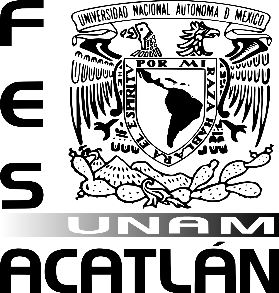
\includegraphics[width=0.15\textwidth]{../auxiliary/assets/fes.png}

        \vspace*{5cm}
        \LARGE
        \textbf{\titulo}

        \vspace{1cm}
        \large
        Camargo Badillo Luis Mauricio \\
        \vspace{1.5cm}

        \vfill

        \vspace{0.5cm}
        Audiciones Fase 3 \\
        \textbf{Programa de Inducción a Matemáticas Aplicadas y Computación}\\
    \end{center}
\end{titlepage}


\tableofcontents
\newpage

Recordemos que una \textbf{ecuación diferencial} es una ecuación que relaciona una (o más) funciones con sus derivadas. Estas ecuaciones son de gran utilidad, pues nos ayudan a modelar muchos fenómenos naturales, el objeto de estudio de muchas disciplinas como la física, la ingeniería, la química, la biología, la astronomía, etc.; las ecuaciones diferenciales también modelan otros fenómenos de la economía y otras ciencias matemáticas. Es por esta razón por la que la resolución de ecuaciones diferenciales es un área de tanto interés en el mundo actual.

Usualmente, al tener una ecuación diferencial, el objetivo es encontrar la función (o las funciones) que la satisfagan. No obstante, dependiendo de la complejidad de la ecuación y de su forma, puede ser difícil o incluso imposible encontrar la solución exacta y explícita de forma analítica, un problema que se presenta sin importar si buscamos la solución manualmente o le asignamos la tarea a una computadora. De hecho, son bastantes las aplicaciones que involucran ecuaciones diferenciales cuya solución no se puede obtener de forma analítica; las ecuaciones que definen la forma del ala de un avión son un ejemplo.

Es por esta problemática por lo que nos apoyamos de los métodos numéricos para resolver este tipo de ecuaciones diferenciales. Recordemos que los métodos numéricos son técnicas que nos ayudan a aproximar procesos matemáticos y que se han vuelto especialmente populares luego del \textit{boom} en poder computacional que se ha experimentado en las últimas décadas; la resolución de esta clase de ecuaciones diferenciales son tan solo una de las muchas aplicaciones de los métodos numéricos.

Evidentemente, dada la naturaleza de los métodos numéricos, no tendremos una solución exacta como la analítica, pero ciertamente podemos tener una solución lo suficientemente cercana como para poder confiar en ella. En el mundo actual, podemos constatar que las soluciones obtenidas son perfectamente válidas: miles de aviones vuelan todos los días a pesar de que las ecuaciones que modelan la aerodinámica deben ser resueltas numéricamente.

Los \textbf{métodos de Runge-Kutta} son algunos de los métodos numéricos más ampliamente utilizados para la resolución de estas ecuaciones diferenciales, dado un problema de valor inicial. Estos métodos proporcionan soluciones más precisas que aquellas dadas por otros métodos numéricos más sencillos, como el método de Euler. A lo largo de este documento, se estará dando un panorama general de estos métodos, sus diferentes tipos y cómo utilizarlos, cerrando con una aplicación.

\section{Introducción a los Métodos de Runge-Kutta}

Los métodos de Runge-Kutta son una familia de métodos numéricos iterativos desarrollados por los matemáticos alemanes Carl Runge y Wilhelm Kutta alrededor de los inicios del siglo XX.\@

Estos métodos tienen como objetivo obtener una curva aproximada a la solución de un problema de valor inicial que involucra una ecuación diferencial \textit{ordinaria}, especialmente cuando se trata del tipo de problemas cuya solución analítica es difícil o imposible de obtener, como ya fue establecido en la introducción de este texto. Debido a su relativamente rápida convergencia en relación a otros métodos, los métodos de Runge-Kutta son ampliamente preferidos, a pesar de que son computacionalmente más demandantes,

De forma similar a otros métodos numéricos utilizados para las ecuaciones diferenciales, los métodos de Runge-Kutta son iterativos, lo que quiere decir que una primera estimación es utilizada para obtener una segunda más precisa y así sucesivamente.

\section{Método de Runge-Kutta de Grado 4}

El método más utilizado de los Runge-Kutta es el de grado 4, frecuentemente conocido como «RK4»; incluso algunas veces es simplemente llamado \textit{el} método de Runge-Kutta.

\subsection{Funcionamiento de RK4}\label{sect:def-rk4}

Sea la siguiente ecuación diferencial:
\begin{equation} \label{eq:main-diff-eq}
	\frac{dy}{dt} = f(t,y)
\end{equation}
…con la condición de valor inicial:
\begin{equation*}
	y(t_0) = y_0
\end{equation*}
Aquí conocemos \(f\) y las condiciones inicales \(t_0, y_0\), deseando aproximar a \(y\), una función desconocida sobre \(t\). Utilizaremos el método RK4 para obtener esta aproximación.

Antes que nada, debemos:
\begin{itemize}
	\item Definir el intervalo para \(t\) sobre el cual estaremos aproximando la solución.
	\item Definir el tamaño \(h\) de los pasos por iteración que estaremos tomando sobre ese intervalo.
\end{itemize}
El número de iteraciones que realizaremos dependerá de la razón entre el intervalo para \(t\) y el tamaño \(h\) que elijamos. Aquí, estamos básicamente convirtiendo el intervalo continuo de \(t\) en uno discreto a través de \(h\), sobre el cual estaremos iterando en el método.

Comenzamos definiendo los dos valores más importantes que se estarán determinando durante cada iteración \(n \in [0, 1, 2, \dots]\):
\begin{align}
	y_{n+1} &= y_{n} + \frac{h}{6} \left( k_{1} + 2k_{2} + 2k_{3} + k_{4} \right) \label{eq:weighted-avg} \\[0.5em]
	t_{n+1} &= t_{n} + h \nonumber
\end{align}
Es en la definición de \(y_{n+1}\) que se nos presentan los valores \(k_{1}, k_{2}, k_{3}, k_{4}\), que son los que caracterizan al método RK4 y donde realizaremos la mayor cantidad de cálculos involucrados. Estos cuatro valores se definen para cada iteración \(n\) como:
\begin{align}
	k_{1} &= f(t_{n}, y_{n}) \label{eq:k1} \\
	k_{2} &= f \left( t_{n} + \frac{h}{2}, y_{n} + h \frac{k_{1}}{2} \right) \label{eq:k2} \\
	k_{3} &= f \left( t_{n} + \frac{h}{2}, y_{n} + h \frac{k_{2}}{2} \right) \label{eq:k3} \\
	k_{4} &= f(t_{n} + h, y_{n} + hk_{3}) \label{eq:k4}
\end{align}

\subsection{Visualización de RK4}

Puede que hasta el momento la descripción anterior del método de Runge-Kutta de grado 4 (RK4) haya parecido bastante abstracta, pero describámosla y visualicémosla para que su funcionamiento quede más claro.

\begin{figure}[H]\label{fig:slopes}
	\centering
	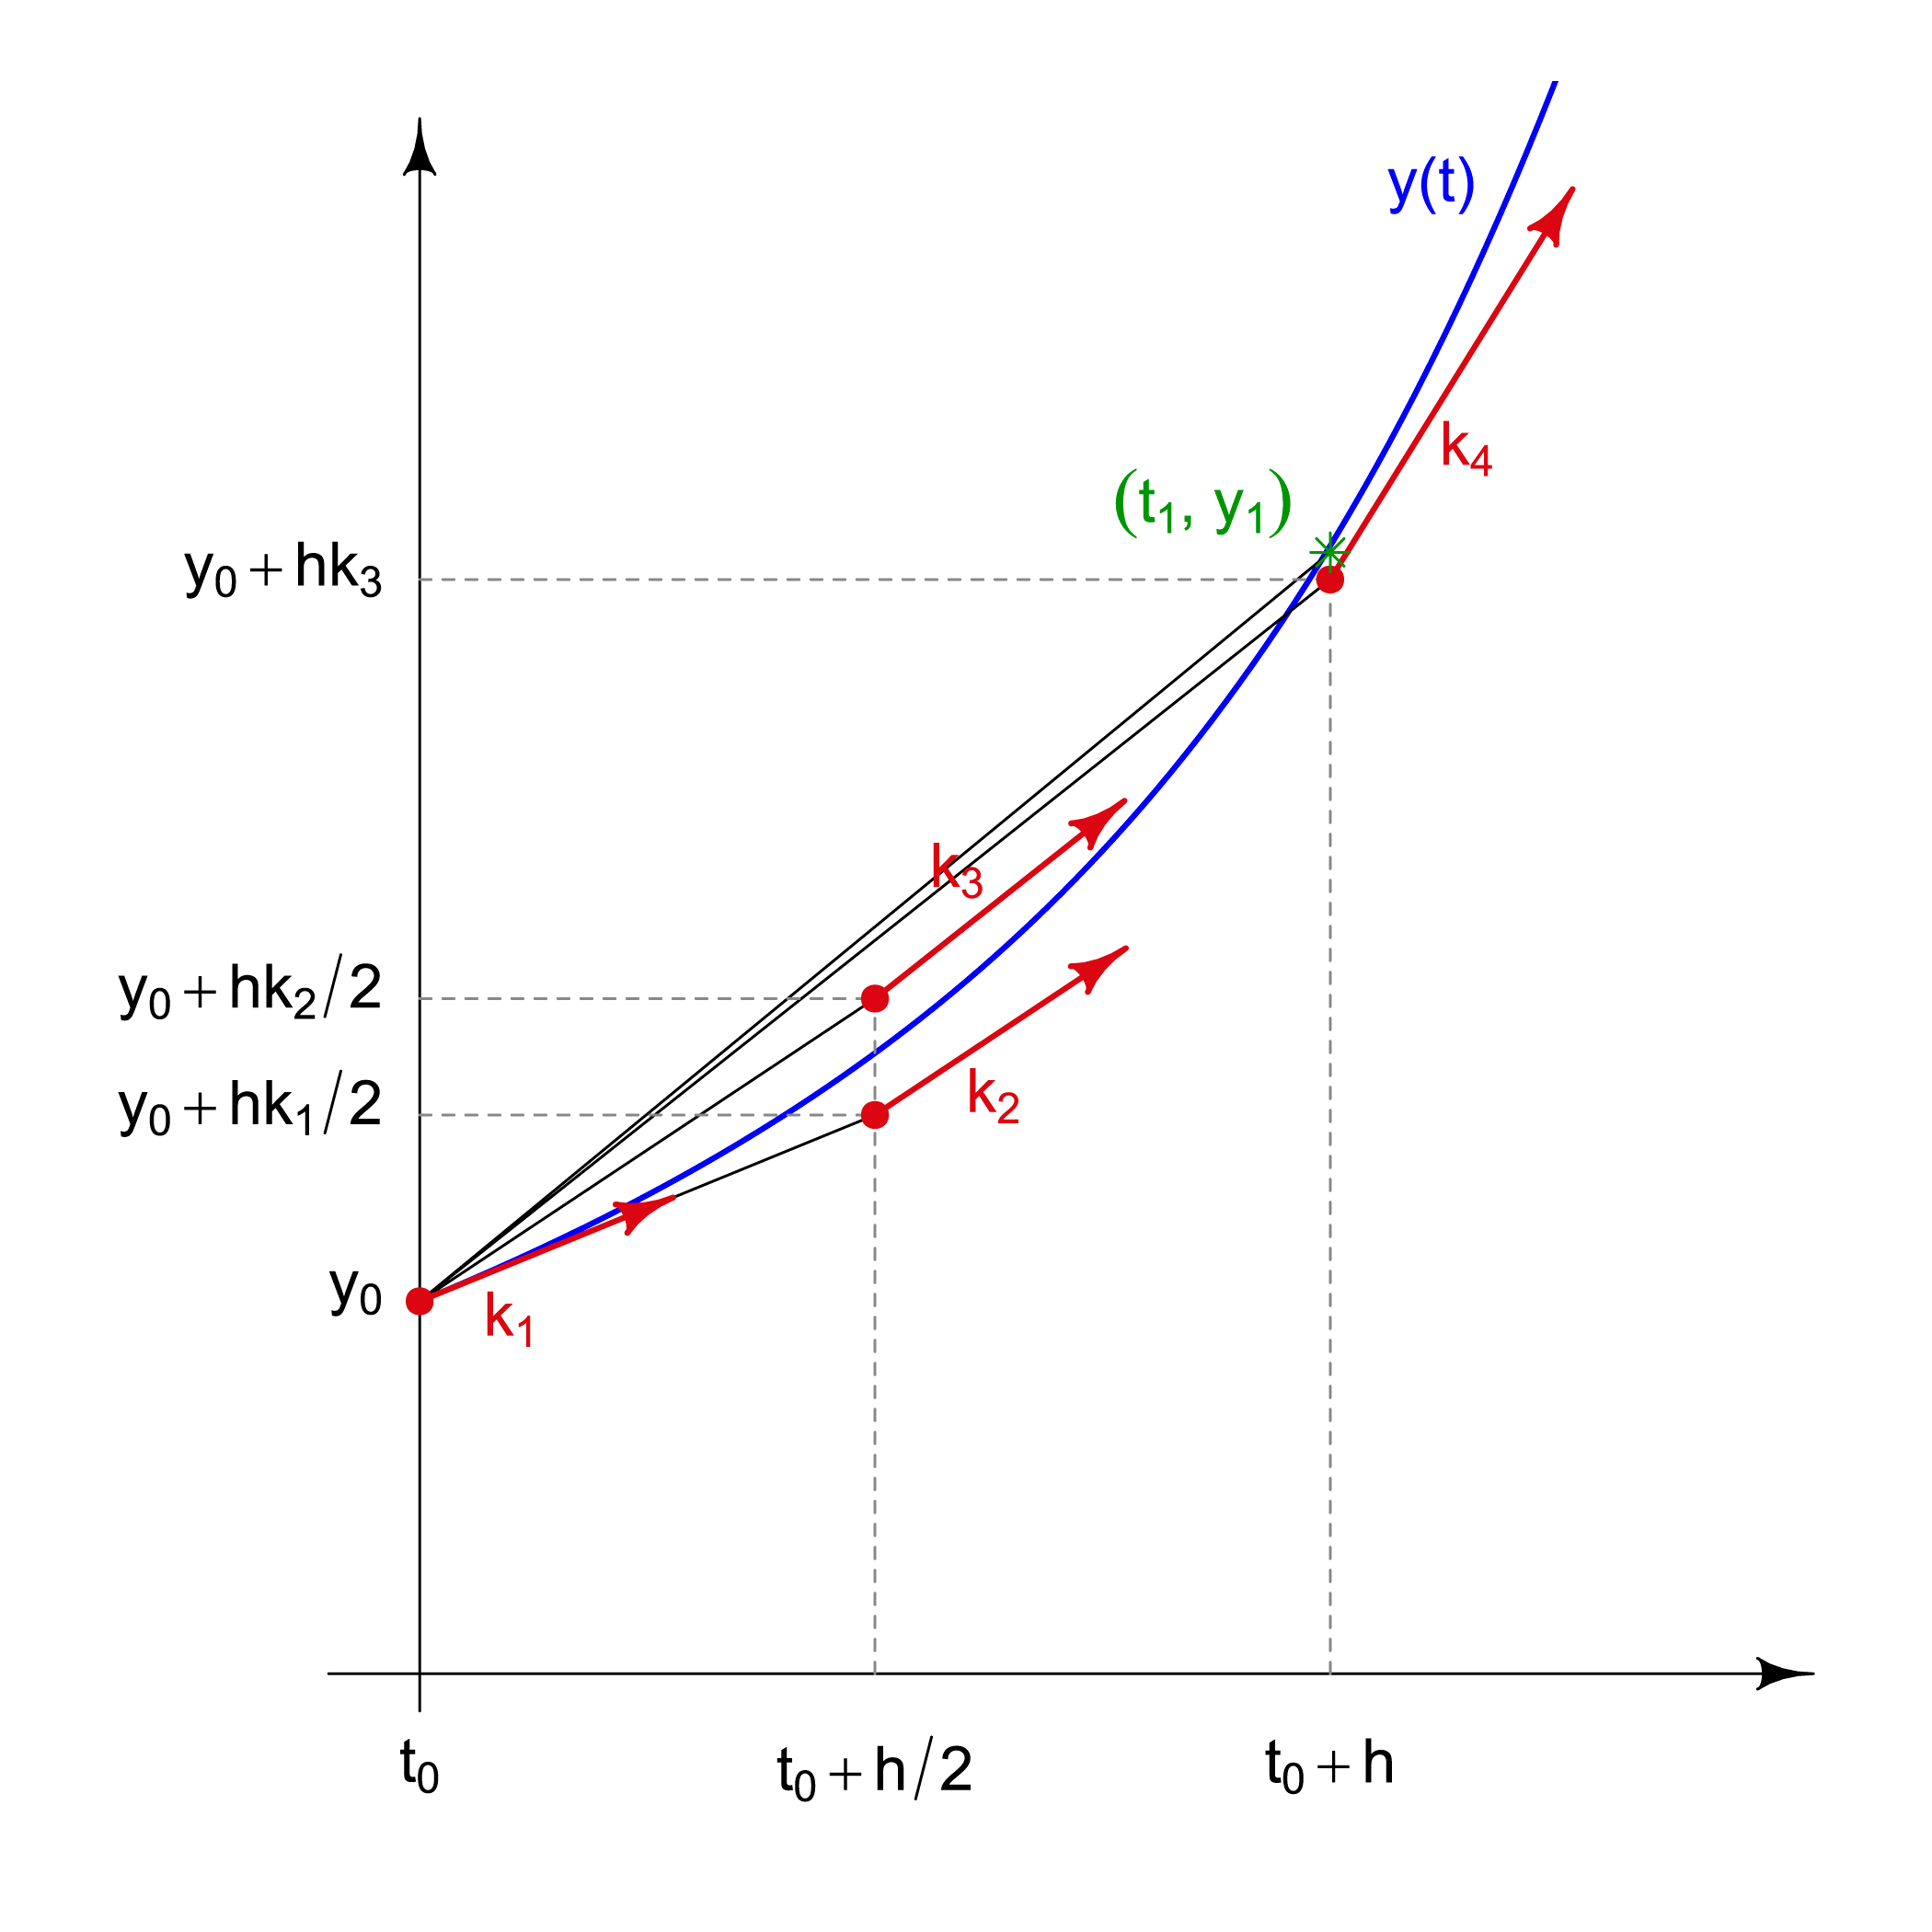
\includegraphics[scale=0.6]{../auxiliary/assets/Runge-Kutta_slopes.png}
	\caption{Aproximación de la solución a \(\frac{dy}{dt} = y + t^{3}\) con \(y_{0}\) y un intervalo para \(t\) arbitrarios. En azul, la solución exacta; en rojo, las pendientes correspondientes a los valores \(k_{i}\); en verde, uno de los puntos de la solución, que corresponde a la aproximación obtenida durante la primera iteración con paso \(h\). Gráfico obtenido de \url{https://en.wikipedia.org/wiki/File:Runge-Kutta_slopes.svg}.}
\end{figure}
La figura~\ref{fig:slopes} representa el funcionamiento de RK4 para la obtención de la solución a la ecuación diferencial \(\frac{dy}{dt} = y + t^{3}\) bajo la condición \(y(t_{0}) = y_{0}\), con \(y_{0}\) y el intervalo para \(t\) arbitrarios.

La obtención analítica de la solución exacta para esta ecuación diferencial es, de hecho, posible y es por ello por lo que pudo ser trazada como la línea azul, por lo que estrictamente hablando no es necesaria la implementación de un método numérico para obtenerla. Sin embargo, se ha utilizado simplemente para ejemplificar y visualizar el funcionamiento del método RK4.

\subsubsection{Pendientes a lo Largo del Intervalo}

Lo primero que notamos es que los valores \(k_{i}\) representan pendientes. Si regresamos a su definición en la sección anterior ((\ref{eq:k1}), (\ref{eq:k2}), (\ref{eq:k3}) y (\ref{eq:k4})), notamos que son simplemente evaluaciones de \(f(t,y)\) en valores concretos para \(t\) y \(y\), y que la ecuación diferencial de la que partimos establece que esa función describe la derivada (véase (\ref{eq:main-diff-eq})), por lo que la razón de ser de este resultado se vuelve evidente.

Analizando un poco más las definiciones de estas \(k_{i}\), y con ayuda de la figura~\ref{fig:slopes}, notaremos también que estas pendientes no son del todo arbitrarias:
\begin{itemize}
	\item \(k_{1}\) es la pendiente al inicio del intervalo.
	\item \(k_{2}\) es la pendiente en el punto medio del intervalo (de ahí que involucre \(\frac{h}{2}\)), apoyándose de \(k_{1}\).
	\item \(k_{3}\), similar a \(k_{2}\), es la pendiente en el punto medio del intervalo, pero esta vez apoyándose de \(k_{2}\).
	\item \(k_{4}\) es la pendiente al final del intervalo
\end{itemize}

\subsubsection{Aproximación Obtenida}

Al final de cada iteración \(n\) obtenemos \(y_{n+1}\), que no es más que la aproximación de \(y(t_{n+1})\) según el método.

Notemos que este valor es determinado por la \(y_{n}\) actual correspondiente a la iteración, sumada con una media ponderada de cuatro incrementos, cada uno correspondiendo al producto de las cuatro pendientes anteriormente descritas por la longitud del paso \(h\). Esta media ponderada favorece sobre todo a las pendientes \(k_{2}\) y \(k_{3}\), las del medio del intervalo.

Visto de otra forma, las pendientes \(k_{i}\) descritas anteriormente van guiando al método a lo largo del intervalo, lo que le permite obtener una aproximación relativamente precisa de un punto de la solución al final de él.

\section{Aplicación de RK4}

Ya se introdujo a los métodos numéricos de Runge-Kutta y se describió el más popular, RK4. A continuación, para seguir con el desarrollo de este método, se describirá una aplicación en la cual este método puede ser aplicado.

\subsection{Oscilador de Van der Pol}

Recordemos que un oscilador es un sistema dinámico que presenta una especie de variación estable y periódica a lo largo del tiempo. Uno de los osciladores más sencillos es el oscilador armónico amortiguado, que es descrito por la siguiente ecuación diferencial ordinaria de segundo orden:
\[
	\frac{d^2 y}{dx^2} + \mu \frac{dy}{dx} + y = 0
\]
Aquí, \(\mu\) es un parámetro escalar que controla el amortiguamiento del sistema (sobreamortiguamiento, amortiguamiento crítico o subamortiguamiento). Las soluciones a esta ecuación diferencial pueden ser obtenidas analíticamente de forma relativamente sencilla, así que no nos enfocaremos en esta aplicación.

En lugar, preferiremos como sujeto de estudio al \textbf{oscilador de Van der Pol}. Este tipo de oscilador, nombrado en honor al físico e ingeniero eléctrico neerlandés Balthasar van der Pol, tiene una amortiguación no lineal, lo que resulta en un comportamiento curioso que a lo largo del tiempo es descrito por la siguiente ecuación diferencial ordinaria de segundo orden:
\begin{equation} \label{eq:van-der-pol}
	\frac{d^2 x}{dt^2} - \mu (1 - x^{2}) \frac{dx}{dt} + x = 0
\end{equation}
…donde \(x\) representa la coordenada de la posición (en función de \(t\)) y \(\mu\) es un parámetro escalar que controla la no linearidad y la fuerza del amortiguamiento. Esta ecuación es algunas veces llamada simplemente la «ecuación de Van der Pol».

Esta ecuación tiene muchas aplicaciones, que van desde la física y la electrónica hasta la biología. Originalmente fue utilizada para describir las oscilaciones de un circuito de tubos de vacío, pero más recientemente ha sido utilizada para describir el comportamiento de las neuronas y para el desarrollo de un modelo que describe la interacción entre dos placas geológicas, solo por citar un par de ejemplos.

Debido a que la ecuación de Van der Pol no es lineal, es imposible la obtención de una solución analítica exacta en términos de funciones elementales conocidas. Por ello, el único camino que tenemos para analizar su solución son los métodos numéricos. Utilizaremos el método RK4 para encontrar numéricamente las soluciones a esta ecuación.

\subsection{Van der Pol en Términos de Ecuaciones de Primer Orden}

Antes de poder utilizar el método de Runge-Kutta de grado 4 para la obtención de las soluciones numéricas de la ecuacióned Van der Pol, debemos notar que no podemos aplicarlo de manera directa sobre la ecuación~(\ref{eq:van-der-pol}), pues, recordemos que, tal como fue descrito en la sección~\ref{sect:def-rk4}, el método necesita de una ecuación de \textit{primer} orden de la forma de~(\ref{eq:main-diff-eq}).

No obstante, podemos establecer \(y = \frac{dx}{dt}\), y así podemos reescribir la ecuación~(\ref{eq:van-der-pol}) como un sistema de dos ecuaciones diferenciales ordinarias de primer orden:
\begin{equation} \label{eq:system-van-der-pol}
	\begin{cases}
		\dfrac{dx}{dt} &= y \\[1em]
		\dfrac{dy}{dt} &= \mu(1 - x^{2})y - x
	\end{cases}
\end{equation}
De esta forma, ya tenemos dos ecuaciones de la forma necesaria para utilizar el método RK4.

\subsection{Solución con RK4}

Para encontrar las soluciones al sistema~(\ref{eq:system-van-der-pol}) se tendrá que resolver cada una de las ecuaciones de forma independiente con valores iniciales distintos para \(x\) y \(y\), pero cuidando que el valor inicial y el intervalo de \(t\), así como el tamaño \(h\) de los pasos, sean los mismos para ambas ecuaciones.

Si bien se podría realizar el procedimiento del método RK4 a mano, es más conveniente el desarrollo de un programa que lo realice computacionalmente, ahorrándonos tiempo y esfuerzo. Después de todo, la utilización de los métodos numéricos para la obtención de soluciones a ecuaciones diferenciales ordinarias (y muchas otras aplicaciones) se ha vuelto especialmente viable en las últimas décadas luego de los avances en la velocidad de procesamiento computacional.

El programa fue realizado en Python, un lenguaje de programación popular para este tipo de aplicaciones. La implementación de RK4 en Python es sumamente sencilla y solo se utilizaron los paquetes \textit{numpy} para un manejo más elegante de los cálculos, y \textit{matplotlib} para la graficación de la solución obtenida.

\begin{lstlisting}[style=python]
import numpy as np
import matplotlib.pyplot as plt

# Retorna la evaluacion segun la ecuacion de Van der Pol
def van_der_pol(x, y, m):
    return [y, m*(1 - x**2)*y - x]

# Aplica RK4 para encontrar las soluciones a Van der Pol
def runge_kutta(t0, x0, y0, m, h, t_final):
    total_steps = int((t_final - t0) / h)

	# Arreglos para la discretizacion de t y los valores de x, y
    t = np.linspace(t0, t_final, total_steps)
    x = np.zeros(total_steps)
    y = np.zeros(total_steps)

    x[0] = x0
    y[0] = y0

	# Aproximacion de los puntos hasta cubrir todos los valores de t
    for i in range(1, total_steps):
		# Pendientes
        k1 = h * np.array(van_der_pol(x[i-1], y[i-1], m))
        k2 = h * np.array(van_der_pol(x[i-1] + 0.5*k1[0], y[i-1] + 0.5*k1[1], m))
        k3 = h * np.array(van_der_pol(x[i-1] + 0.5*k2[0], y[i-1] + 0.5*k2[1], m))
        k4 = h * np.array(van_der_pol(x[i-1] + k3[0], y[i-1] + k3[1], m))

		# Aproximacion del punto siguiente
        x[i] = x[i-1] + (1/6) * (k1[0] + 2*k2[0] + 2*k3[0] + k4[0])
        y[i] = y[i-1] + (1/6) * (k1[1] + 2*k2[1] + 2*k3[1] + k4[1])

    return t, x, y

# Grafica la solucion
def plot_solution():
    fig, (ax1, ax2) = plt.subplots(1, 2, figsize=(15, 5))

    # Grafica 1: x, y contra t
    ax1.plot(t, x, label="x(t)")
    ax1.plot(t, y, label="y(t)")
    ax1.set_xlabel("t")
    ax1.set_ylabel("x, y")
    ax1.legend()
    ax1.grid(True)
    ax1.set_title("Solucion para x, y de Van der Pol con RK4; independientes")

    # Grafica 2: x contra y
    ax2.plot(x, y, label="Trayectoria")
    ax2.set_xlabel("x")
    ax2.set_ylabel("y")
    ax2.set_title("Solucion para x, y de Van der Pol con RK4; conjuntas")
    ax2.legend()
    ax2.grid(True)

    plt.tight_layout()
    plt.show()

# Definicion de mu, h y valores iniciales
# m = 1.0
# x0 = 1.0
# y0 = 0.0
# t0 = 0
# t_final = 50
# h = 0.01

m = float(input("- Introduce el valor del parametro mu: "))
x0 = float(input("\n- Introduce el valor inicial x_0 para x: "))
y0 = float(input("- Introduce el valor inicial y_0 para y: "))
t0 = float(input("\n- Introduce el valor inical t_0 para t: "))
t_final = float(input("- Introduce el valor final que tomara t: "))
h = float(input("\n- Introduce el tamano h de los pasos: "))

# Resolucion con RK4 y graficacion
t, x, y = runge_kutta(t0, x0, y0, m, h, t_final)
plot_solution()
\end{lstlisting}

\section{Conclusión}

\end{document}
